\documentclass[10pt]{article}
\usepackage[margin=0.82in]{geometry}
\usepackage{booktabs,amsmath,graphicx,hyperref,xcolor}
\hypersetup{colorlinks=true,linkcolor=blue!50!black,urlcolor=blue!50!black}
\title{Progressive Retrieval Attention with Ollama:\\
Transparent Context Optimization for Local-Model Applications}
\author{Jorge Sim\~ao}
\date{September 2026}

\begin{document}
\maketitle

\begin{abstract}
Ollama combines local-model packaging, lifecycle management, and a stable
application API. Progressive Retrieval Attention (PRA) should preserve that
product surface: ordinary installations receive selected-text E0, while a
PRA-aware model backend may negotiate native E2 without requiring a second
attention implementation in Ollama. We implement this capability-negotiated
adapter, pin a current source audit, and test Windows and Apple Metal daemons.
In a Qwen3-8B M5 replication over 15 natural-QA examples, selected prompts used
10.0--42.2\% of full-context tokens. Median time to first token decreased from
1328 to 1129 ms on HotpotQA and from 2533 to 929 ms on QASPER; 2Wiki again
reversed direction under warm reuse. Keeping Qwen3-8B alive reduced request
latency from 5.84 s cold to 0.714 s across five warm requests
(8.18$\times$). No native backend
handshake was available, so AUTO correctly remained E0. The result is a usable
gateway integration and a precise delegation boundary, not an Ollama-native E2
claim.
\end{abstract}

\section{Introduction}
Ollama's value is operational simplicity: a model name, one daemon, and a
familiar API. A PRA integration that requires every application to understand
engine-specific K/V state would undermine that value. We instead treat Ollama
as the product and model-lifecycle layer. PRA owns typed records,
authorization, selection, sessions, and storage policy. The active model runner
owns attention and physical cache state.

This division creates one hard rule: deeper support is negotiated, never
inferred from a version string or from Ollama's historical relation to a
particular backend. Current Ollama may select different runners for different
models and platforms. An application-facing adapter must therefore be able to
downgrade safely.

Our contributions are an Ollama-native HTTP adapter, a model-fingerprint
invalidation rule, optional backend delegation, live selected-text and lifecycle
measurements, and tests that keep the advertised integration level honest.

\section{PRA Levels and Ownership}
E0 serializes selected evidence into visible messages. E1 transports logical
resource identities without changing attention. E2 consumes detached selected
native K/V. E3 additionally requires scheduler-owned placement, sharing,
prefetch, and eviction. The adapter reports the deepest implemented level, not
the deepest level described by the protocol.

\begin{figure}[t]
\centering
\fbox{\begin{minipage}{0.92\linewidth}\small
Existing Ollama client $\rightarrow$ PRA gateway/SDK $\rightarrow$ capability
probe.\\[2pt]
No native handshake $\rightarrow$ selected records become an ordinary system
message $\rightarrow$ \texttt{/api/chat} (E0).\\[2pt]
Validated backend handshake $\rightarrow$ resource/version/model fingerprint
$\rightarrow$ backend-native PRA executor (E2/E3).\\[2pt]
Unload or model switch $\rightarrow$ invalidate incompatible native state;
Ollama continues to own runner load, keep-alive, and scheduling.
\end{minipage}}
\caption{Gateway-first integration. Native support is inherited from the active
backend rather than reimplemented in Ollama.}
\label{fig:architecture}
\end{figure}

\section{Pinned Architecture Audit}
The source audit pins Ollama commit
\texttt{e37a00a8fa94fca07cefd544bffc9d8997ebcd44}. The measured daemon is version
0.6.8; these are recorded separately because behavior observed in one must not
be projected onto the other. The audited code exposes chat/generate, model
inspection, installed/running model lists, keep-alive, and runner scheduling.
Backend choice is an implementation decision, so the PRA capability cannot be
deduced from the model package alone.

The public API exposes useful timing counters: load, prompt evaluation, token
evaluation, and total duration. It does not expose a detached semantic K/V
contract. Thus the stock daemon qualifies at E0. A future Ollama integration can
reach E2 by delegating to a backend adapter with model/resource identity and
native attention support; it should not duplicate backend kernels in the
product layer.

\section{Implementation}
\texttt{OllamaEngineAdapter} calls \texttt{/api/show} before execution and hashes
the model name, modification metadata, details, and model information. A model
change invalidates state held by an optional native backend executor. In E0,
selected resources are inserted as an ordinary system message with explicit
resource IDs and URIs, then sent to \texttt{/api/chat}. Tool schemas and the
request's generation bound are preserved. Reasoning is an explicit adapter
option and defaults off for bounded answer generation. Ollama 0.30.8 honors
\texttt{think=false} on its native endpoint; its OpenAI-compatible endpoint
ignored that extension in our run, so the benchmark also sends Qwen's
\texttt{/no\_think} control. A regression test protects both the request field
and prompt control and verifies that the caller's messages are not mutated.

\texttt{inspect\_endpoint()} queries \texttt{/api/version}, \texttt{/api/tags},
and \texttt{/api/ps}. The runtime provider's doctor reports the endpoint and
models but labels native PRA as fallback unless a backend handshake is supplied.
\texttt{unload()} uses Ollama's zero keep-alive request and invalidates delegated
state. Unit tests cover E0 injection, endpoint inspection, metrics preservation,
and the rule that only explicit backend delegation upgrades to E2.

\section{Experimental Method}
We ran Ollama 0.6.8 on Windows 10 with Qwen2.5-0.5B. The natural cohort freezes
the evidence selection and compares no context, selected text up to 384 source
tokens, and full text up to 1024 source tokens. It contains five examples each
from HotpotQA, QASPER, and 2WikiMultiHopQA, with two repeats and 16 generated
tokens. Streaming HTTP measurements provide TTFT and inter-token latency.

The lifecycle experiment unloads Qwen, runs one cold and five keep-alive
requests, switches to SmolLM2-135M, unloads it, and returns to Qwen. The selected
record and query remain fixed. This isolates model lifecycle from retrieval.
The cohort is a smoke calibration and does not support production tail-latency
or model-quality claims.

A second host is an Apple M5 with 10 CPU and 10 GPU cores and 16 GB unified
memory, running Ollama 0.30.8 and the official Qwen3-8B Q4\_K\_M GGUF. The
larger-model cohort uses the same 15 identities and frozen selections, a
384-token selected cap, a 4096-token full cap, two repeats, and 12 generated
tokens. Its separate lifecycle run unloads Qwen3-8B, executes five warm
requests, switches to SmolLM2-135M, and returns to Qwen. The first SmolLM use
includes Metal runner compilation and is therefore a deployment observation,
not model-scale evidence.

\section{Results}
\begin{table}[t]
\centering\small
\caption{Natural E0 qualification on Ollama. Prompt ratio is selected/full;
TTFT is median ms; F1 is selected/full.}
\begin{tabular}{lrrr}
\toprule Dataset & Prompt ratio & TTFT selected/full & F1 selected/full\\
\midrule
HotpotQA & 0.410 & 348.6 / 602.8 & 0.404 / 0.314\\
QASPER & 0.375 & 300.0 / 732.7 & 0.217 / 0.099\\
2Wiki & 0.517 & 309.2 / 263.3 & 0.036 / 0.136\\
\bottomrule
\end{tabular}
\label{tab:e0}
\end{table}

\begin{table}[t]
\centering\small
\caption{Qwen3-8B Q4\_K\_M on M5 Metal. Prompt ratio is selected/full; TTFT is
p50 ms; F1 is selected/full.}
\begin{tabular}{lrrr}
\toprule Dataset & Prompt ratio & TTFT selected/full & F1 selected/full\\
\midrule
HotpotQA & 0.327 & 1129 / 1328 & 0.381 / 0.181\\
QASPER & 0.100 & 929 / 2533 & 0.113 / 0.108\\
2Wiki & 0.422 & 984 / 844 & 0.195 / 0.200\\
\bottomrule
\end{tabular}
\label{tab:m5-8b}
\end{table}

Selected text substantially reduces visible context. It also improves TTFT and
token F1 on HotpotQA and QASPER in this run. The 2Wiki reversal is equally
important: the frozen selector's evidence and a small-model generation cap are
not uniformly sufficient. E0 input compression is measured; universal quality
preservation is not.

The 8B replication preserves the same qualitative boundary at a more realistic
local-model scale. Selected text removes 57.8--90.0\% of visible prompt tokens.
It lowers median TTFT by 14.9\% on HotpotQA and 63.3\% on QASPER; 2Wiki is
16.6\% slower at the median, while its full-context p95 reaches 2534 ms versus
1528 ms selected. F1 is approximately preserved on QASPER and 2Wiki and higher
on the five Hotpot examples. Repeats contribute latency samples, not independent
quality samples, so these signs remain smoke evidence.

\begin{table}[t]
\centering\small
\caption{Lifecycle measurements. Warm is the mean of five keep-alive requests.}
\begin{tabular}{lrrr}
\toprule Event & Total ms & Load ms & Prompt-eval ms\\
\midrule
Qwen cold after unload & 2300.5 & 1500.6 & 329.9\\
Qwen warm mean & 506.5 & 30.4 & 5.9\\
Switch to SmolLM2 & 5248.7 & 4465.3 & 248.3\\
Return to Qwen & 503.2 & 36.1 & 5.7\\
\bottomrule
\end{tabular}
\label{tab:lifecycle}
\end{table}

For Qwen3-8B on M5, cold-after-unload latency was 5836 ms and the five warm
requests averaged 713.5 ms, an 8.18$\times$ reduction. All six returned the
selected access code. The first SmolLM2 request took 40.20 s, dominated by
39.38 s reported load time; returning to Qwen took 753 ms. This one-time
alternate-runner result should not be folded into steady-state PRA latency.

\begin{figure}[t]
\centering
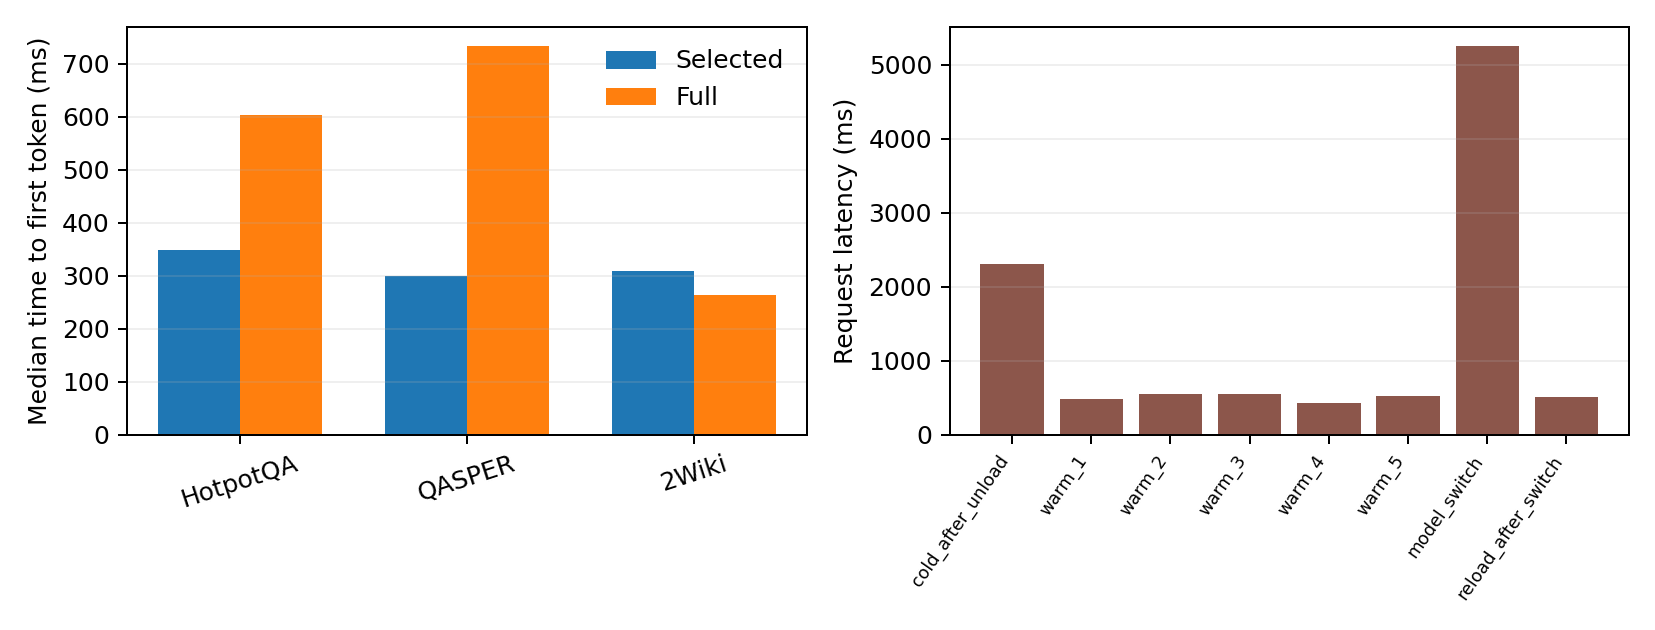
\includegraphics[width=0.97\linewidth]{figures/ollama_qualification.png}
\caption{Selected/full context pressure (left) and model lifecycle (right).
Ollama's keep-alive benefit is large enough that lifecycle state must be
reported separately from PRA selection.}
\label{fig:results}
\end{figure}

The warm mean is 4.54$\times$ faster than the initial cold request. Most of the
difference is model load and prompt evaluation, not PRA logic. The switch test
also shows why the adapter binds native state to a model fingerprint. Returning
to Qwen was warm in this daemon configuration, but an adapter cannot assume
that a runner survives every memory-pressure or scheduling event.

\section{Deployment Matrix}
\begin{table}[h]
\centering\small
\caption{Current product status.}
\begin{tabular}{llll}
\toprule Mode & Transport & Status & Claim\\
\midrule
E0 selected & Ollama/OpenAI HTTP & measured & supported default\\
E1 logical & optional envelope & interface only & no native effect\\
E2 native & delegated backend & not negotiated & AUTO falls back\\
E3 scheduler & Ollama runner & not implemented & no claim\\
\bottomrule
\end{tabular}
\end{table}

This design keeps ordinary clients compatible. An application can point the PRA
gateway at Ollama today. If a future active backend reports E2, the same wire
request can carry stable identities while the backend performs native
materialization. If the handshake disappears after an upgrade or model switch,
AUTO returns to E0.

\section{Limitations and Next Work}
The original Windows runtime is old relative to the pinned source audit; the
paper does not merge those observations with the separate 0.30.8 M5
replication. Two model sizes and hosts are measured, but both cohorts are small.
Memory use, concurrent requests, cancellation, reconnects, daemon
restart, quantized variants, and native E0/E2 parity remain open. The next step
is to expose the same capability handshake through a PRA-aware llama.cpp or
other active backend, then rerun frozen-selection quality and lifecycle tests
without changing the client.

\section{Conclusion}
Ollama can provide a low-friction PRA entry point without becoming a second PRA
runtime. The measured E0 path reduces visible context at both 0.5B and 8B and
benefits two of three small natural-QA slices; keep-alive dominates cold
latency. Native support must
be delegated and negotiated. On the tested daemon it was absent, and the safe
fallback worked as designed.

\section*{Artifact Availability}
Branch \texttt{research/paper6-8-ollama} contains the adapter, tests, raw JSON,
lifecycle benchmark, plot generator, README, and manuscript.

\begin{thebibliography}{9}
\bibitem{ollama} Ollama contributors. \emph{Ollama}.
\url{https://github.com/ollama/ollama}
\bibitem{openai} OpenAI. \emph{Chat Completions API}.
\url{https://platform.openai.com/docs/api-reference/chat}
\bibitem{qwen25} Qwen Team. \emph{Qwen2.5 Technical Report}. 2024.
\url{https://arxiv.org/abs/2412.15115}
\end{thebibliography}
\end{document}
